\section{Produktdesign}

\subsection{Login}
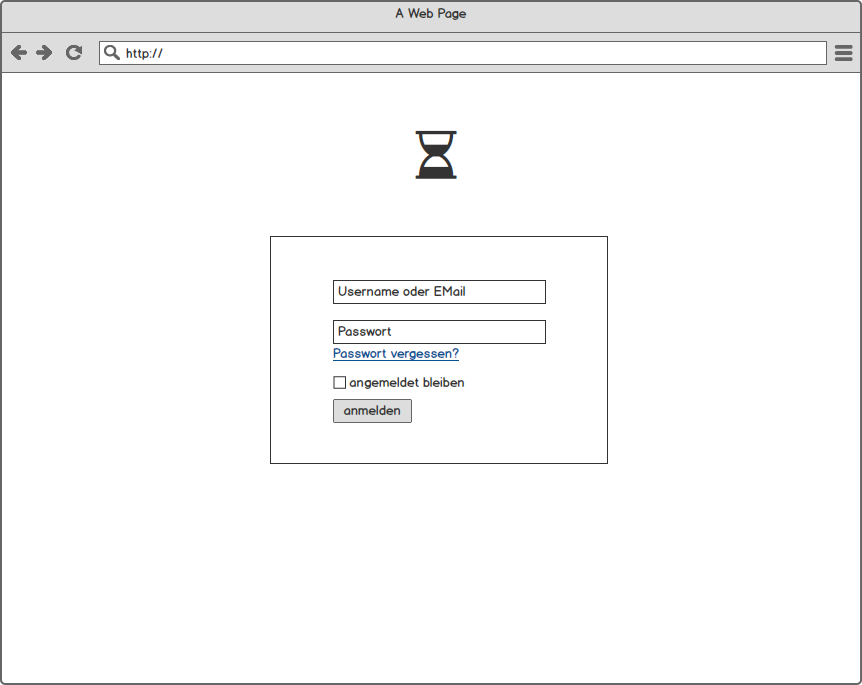
\includegraphics[width=\linewidth]{UI/Login/Login.png}

\newpage
\subsection{Benutzer*}

\textbf{\\Neue Zeiterfassung}\\
\\
Das ist die Hauptseite vom \emph{Benutzer*}, wo dieser direkt nach einer erfolgreichen Anmeldung oder durch Drücken auf die Schaltfläche "neue Zeiterfassung" geleitet wird. \\
Um eine neue \emph{Zeiterfassung} zu starten, wählt der \emph{Benutzer*} eine \emph{Kategorie} und eine \emph{Tätigkeit} aus, anschließend drückt er auf den Start Button. Der \emph{Benutzer*} kann die Zeiterfassung über den Stop Button beenden.\\
\\
\\
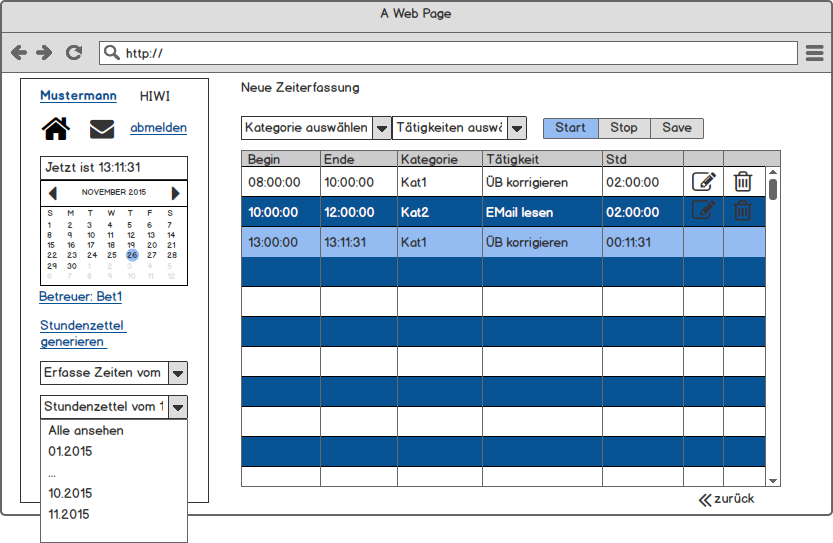
\includegraphics[width=\linewidth]{UI/Benutzer/Zeiterfassung.png}


\newpage
\textbf{\\Erfasste Zeiten bearbeiten}\\
\\
Das ist die Seite fürs Editieren der erfassten Zeiten vom \emph{Benutzer*}.
Es kann entweder direkt von der Seite "Neue Zeiterfassung" über den Edit Button 
\includegraphics[scale=.1]{UI/Button/Edit.png} oder durch auswählen vom Datum auf der Kalenderübersicht auf die linken Seite auf dieser Seite weitergeleitet werden. Nur die erfassten Zeiten, die noch nicht an den Betreuer abgegeben sind, könnten editiert werden.\\
Der \emph{Benutzer*} klickt in das Textfeld, wo er eine Änderung tätigen will, und ändert die dort eingetragene Daten. Anschließend klickt er auf das Save Button 
\includegraphics[scale=.1]{UI/Button/Save.png}, um die Änderungen zu bestätigen.\\
\\
\\
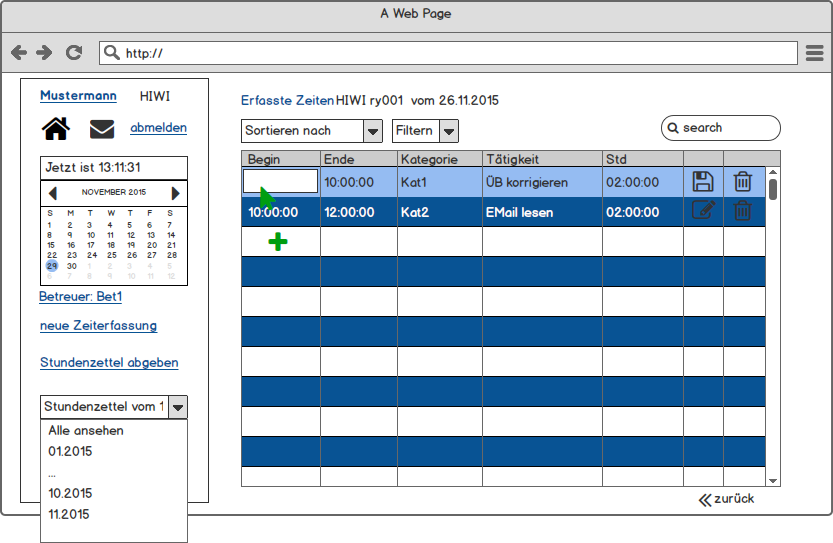
\includegraphics[width=\linewidth]{UI/Benutzer/Editieren.png}





\newpage
\textbf{\\Nachricht Interface vom Benutzer*}\\
\\
Die Nachrichten(Warnungen und Erinnerungen) sieht der \emph{Benutzer*}, indem er auf den Nachricht-Button

\includegraphics[scale=.4]{UI/Button/Nachricht.png} drückt.\\
Die Anzahl der Nachrichten erscheint in dem kleinen Kreis rechts oben auf dem Button.\\
\\
\\
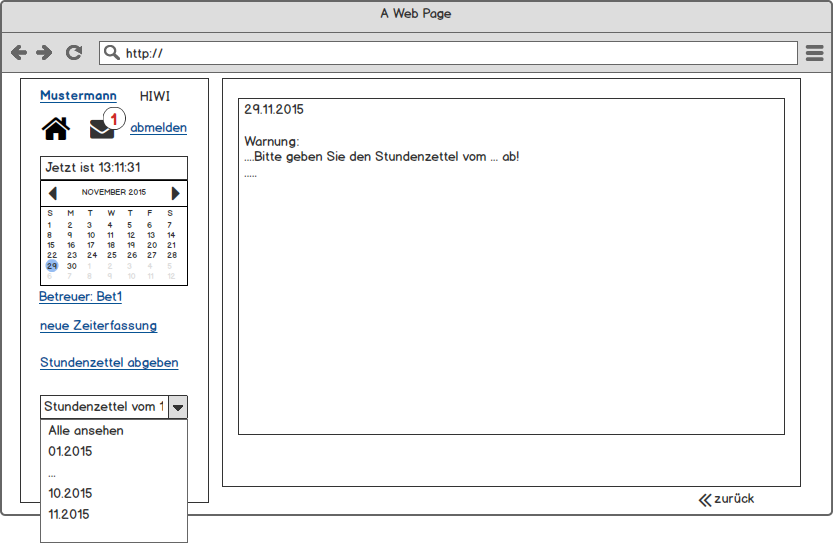
\includegraphics[width=\linewidth]{UI/Benutzer/Nachricht.png}

\newpage
\subsection{Betreuer*}
\textbf{\\Hauptseite vom Betreuer*}\\
\\
Nach der erfolgreichen Anmeldung befindet sich der \emph{Betreuer*} auf dieser Seite.\\
Alle ihm zugewiesenen \emph{Benutzer*} werden samt deren Informationen und Daten angezeigt.\\
Der \emph{Betreuer*} kann hier die schon abgegebenen \emph{Stundenzettel} aufrufen, kontrollieren und ausdrucken.\\
Wenn der \emph{Stundenzettel} korrekt ist, drückt der \emph{Betreuer*} auf "Geprüft". Danach wird der \emph{Administrator*} darüber informiert.\\
Wenn der \emph{Stundenzettel} nicht korrekt ist, drückt der \emph{Betreuer*} auf "Nicht OK". Dann erscheint ein Textfeld, in dem der \emph{Betreuer*} die Gründe der Ablehnung erläutern kann.\\
\\
\\
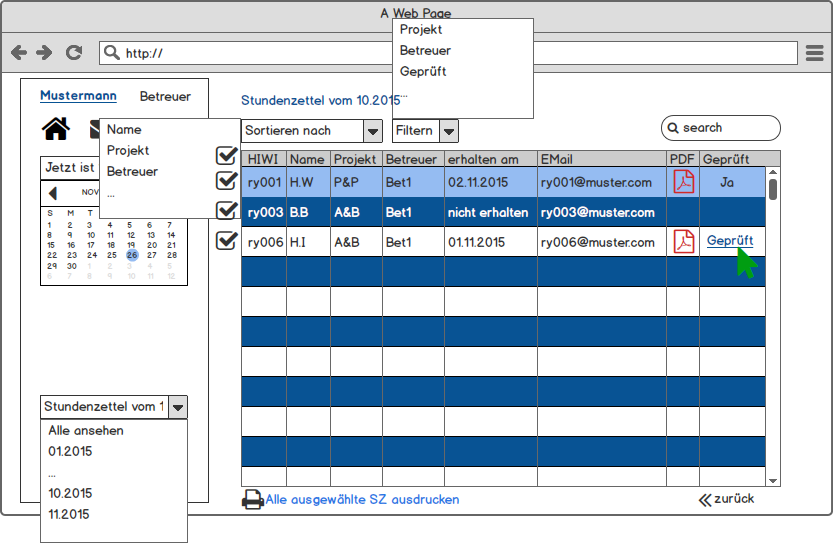
\includegraphics[width=\linewidth]{UI/Betreuer/Hauptseite.png}

\newpage
\textbf{\\Nachricht Interface vom Betreuer*}\\
\\
Auf der Nachrichtenseite wird der \emph{Betreuer*} über Erinnerungen/Warnungen an allen ihm zugewiesenen \emph{Benutzern*} und Abgabe von \emph{Stundenzettel} informiert.\\
Hier kann der \emph{Betreuer*} direkt die \emph{Stundenzettel} aufrufen, kontrollieren und Kommentar dazu schreiben.\\
\\
\\
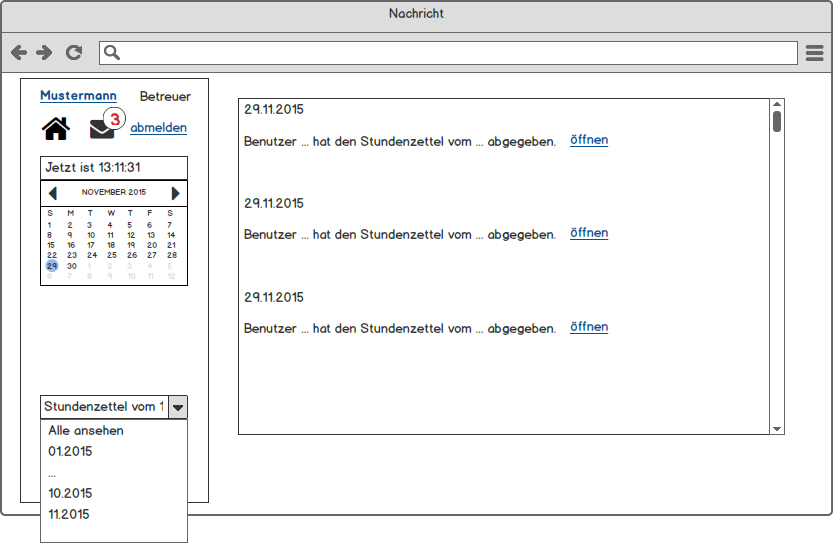
\includegraphics[width=\linewidth]{UI/Betreuer/Nachricht.png}

\newpage
\subsection{Administrator*}
\textbf{\\Hauptseite vom Administrator*}\\
\\
Auf der Hauptseite des \emph{Administrators*} befindet sich die Liste aller \emph{Benutzer*}. Hier wird angezeigt, ob der \emph{Benutzer*} seinen \emph{Stundenzetteln} vom letzten Monat vom \emph{Betreuer*} erfolgreich kontrolliert hat oder nicht.\\
Falls ja wird die Status als "abgegeben" angezeigt und der \emph{Stundenzettel} stehen ebenfalls als PDF-Datei zur Verfügung.\\
Falls nein wird die Status als "nicht abgegeben" angezeigt.\\
Der \emph{Administrator*} kann alle verfügbare \emph{Stundenzettel} auf einmal ausdrucken.\\
Der \emph{Administrator*} kann zur Betreuer*ansicht wechseln, indem er auf den Namen des jeweiligen \emph{Betreuers*} anklickt.\\
\\
\\
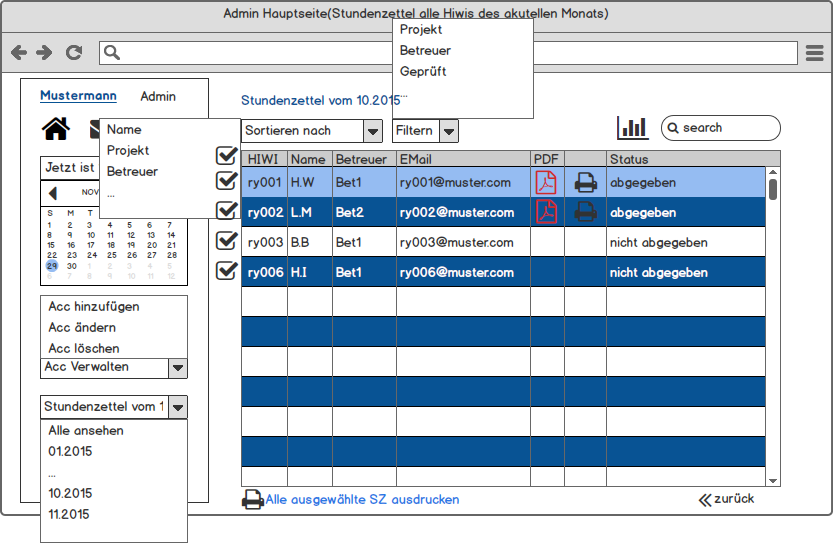
\includegraphics[width=\linewidth]{UI/Admin/Hauptseite.png}

\newpage
\textbf{\\Klickt auf einen einzelnen Benutzer*}\\
\\
Wenn der \emph{Administrator*} sich auf seinem Hauptseite befindet und dort auf einen Namen eines \emph{Benutzers*} klickt, landet er auf die Seite eines einzelnen \emph{Benutzers*}.\\
Der \emph{Administrator*} hat die Möglichkeit zu prüfen, wieviele Stunden  der \emph{Benutzer*} in den jeweiligen vergangenen Monaten arbeiteten und wieviele Stunden sie tatsächlich gearbeitet haben.\\
Außerdem hat der \emph{Administrator*} die Möglichkeit, eine grafische Darstellung der Arbeitsstunden des \emph{Benutzers*} einzusehen.\\
\\
\\

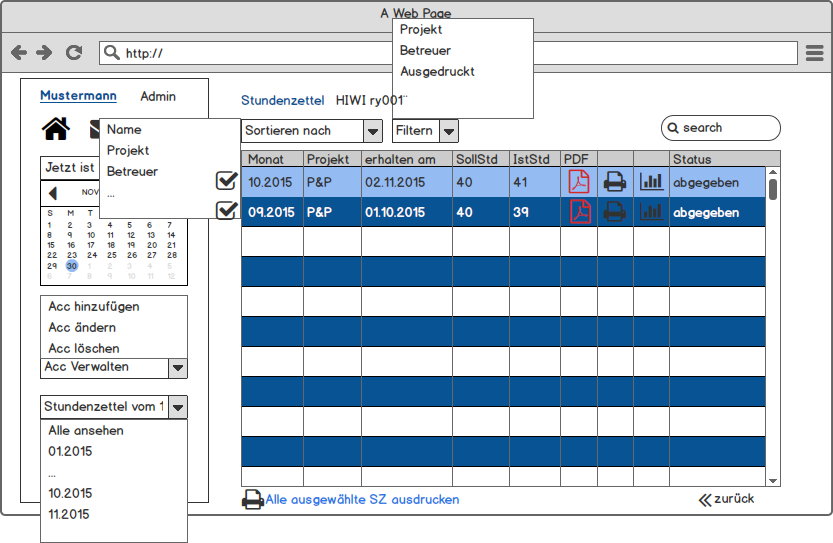
\includegraphics[width=\linewidth]{UI/Admin/EinBenutzer.png}

\newpage
\textbf{\\Account löschen}\\
\\
Der \emph{Administrator*} kann auf dieser Seite den Account vom \emph{Benutzer*} oder \emph{Betreuer*} durch die Sortier- bzw. Filterfunktion bequem finden und löschen.\\
\\
\\
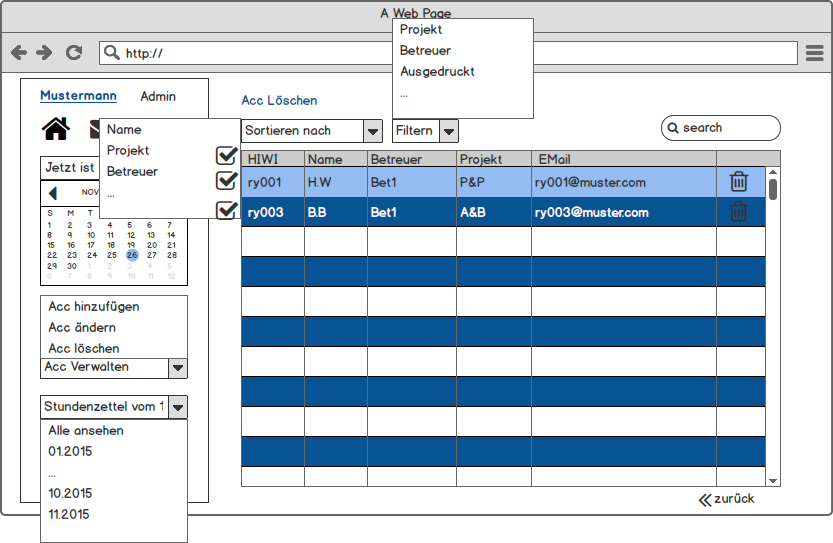
\includegraphics[width=\linewidth]{UI/Admin/Accounts/Ubersicht.png}



\newpage
\textbf{\\Account bearbeiten}\\
\\
Hier hat der \emph{Administrator*} die Möglichkeit, Accounts anderer \emph{Benutzer*} zu bearbeiten.\\
\\
\\
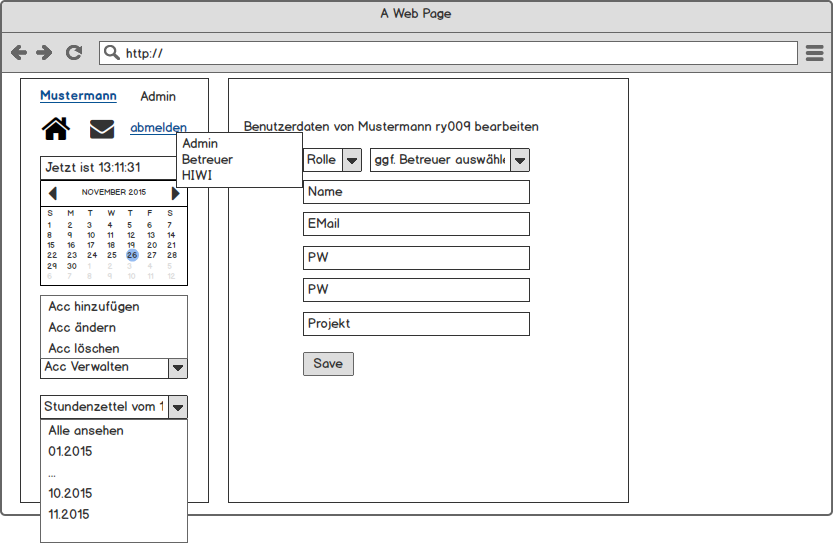
\includegraphics[width=\linewidth]{UI/Admin/Accounts/Bearbeiten.png}
